%% Beamer-ported version of mru.tex ==
%% 
%% Original created 05-10-2008; ported to Beamer July 2025
\documentclass{beamer}


\usepackage{xcolor}
\usetheme{Copenhagen}  % Change to Madrid, Copenhagen, etc., for fancier look
% Define custom colors
\definecolor{electricblue}{RGB}{0,191,255} % Electric blue
\definecolor{creamyblue}{RGB}{173,216,230} % Creamy blue
\newcommand{\red}[1]{\textcolor{red}{#1}}
%\setbeamercolor{structure}{fg=electricblue} % Apply electric blue
\setbeamercolor{structure}{fg=creamyblue} % Apply creamy blue

\usepackage[latin1]{inputenc}
\usepackage{amsmath}
\usepackage{cancel}
\usepackage{tikz}
\usepackage{graphicx}  % For images


%%%%%%%%%%%%%%%%%%%%%%%%%%%%%%%%%%%%%
%% Seguridad.. %%%%%%%%%%%%%%%%%%%%%%
\hypersetup{
pdfpagemode={FullScreen},
pdftitle={MRU e2: ver1},
pdfauthor={mmatex.com},
pdfcreator={mmatex.com},
pdfproducer={mmatex.com},
pdfkeywords={Movimiento,Rectilineo,Uniforme}}
%%%%%%%%%%%%%%%%%%%%%%%%%%%%%%%%%%%%%
%%%%%%%%%%%%%%%%%%%%%%%%%%%%%%%%%%%%%

%% You can insert definicions here..

%% DEFINICIONES MIAS..
%\def\psPiFour{12.566371}
%\def\psPiTwo{6.283185}
\def\psPi{3.14159265}
%\def\psPiH{1.570796327}
%\newdimen\pstRadUnit
%\newdimen\pstRadUnitInv
%\pstRadUnit=1.047198cm % this is pi/3
%\pstRadUnitInv=0.95493cm % this is 3/pi

%% Libreria de formulas %%%%%%%%%%%%%%%%%%%%%%%%%%%%%%%%%%%%
\input{lib/FORMULAS}
%% Libreria de Notas    %%%%%%%%%%%%%%%%%%%%%%%%%%%%%%%%%%%%
\input{lib/NOTASUNIDADES}
%%%%%%%%%%%%%%%%%%%%%%%%%%%%%%%%%%%%%%%%%%%%%%%%%%%%%%%%%%%%

%% Titulo y autor .. obligatorio..
\title{MRU e21: ver1}
\subtitle{Otono - 2025}
\author{mmatex}


%%%%%%% Para pegar el log.. %%%%%%%%%%%%%%%%%%%%%%%%%%%%%%%
\logo{%
    \begin{tikzpicture}
        \node[opacity=0.2] {
\includegraphics[width=1cm]{images/citlogogrey.eps}}; % Use absolute path if needed: /Users/josem/Dropbox/Yachay2024/fisica1/eJJRv1/libs/figs/citlogogrey.eps
    \end{tikzpicture}
}
%%%%%%%%%%%%%%%%%%%%%%%%%%%%%%%%%%%%%%%%%%%%%%%%%%%%%%%%%%%

%%%%%%%%%%%%%%%%%%%%%%%%%%%%%%%%%%%
%%% Comienzo del documento.. %%%%%%
%%%%%%%%%%%%%%%%%%%%%%%%%%%%%%%%%%%
\begin{document}
\maketitle
%%%%%%%%%%%%%%%%%%%%%%%%%%%%%%%%%%

%________________________________________________________________(ult. col, 65)
% ========================== slide1 ============================= 
\begin{frame}
\frametitle{Movimiento Rectil\'ineo Uniforme}
% 
% -Paragraph1 
%----------------------------------------------------------------
%----------------------------------------------------------------
% -Idea1 
% ============================================================== 
 La f\'ormula principal:

                                                               
% ============================================================== 
% -Idea2 
% ============================================================== 
 
{\huge \vmru}
\vNUa
                                                               
% ============================================================== 
% -Idea3 
% ============================================================== 
                                                               
                                                               
                                                               
% ============================================================== 
%----------------------------------------------------------------
%----------------------------------------------------------------
\end{frame}

%________________________________________________________________(ult. col, 65)
% ========================== slide2 ============================= 
\begin{frame}
\frametitle{MRU}
% 
% -Paragraph1 
%----------------------------------------------------------------
%----------------------------------------------------------------
% -Idea1 
% ============================================================== 

Recu\'erdalo por sus unidades:

% ============================================================== 
% -Idea2 
% ============================================================== 

\begin{equation*}
10\frac{\text{km}}{\text{h}} =
\frac{\text{Se recorren 10 km (\red{distancia})}}
{\text{en 1 hora (\red{tiempo})}}
\end{equation*}
                                                               
% ============================================================== 
% -Idea3 
% ============================================================== 
 
Las otras dos f\'ormulas que se derivan de (\ref{vmru}) son:

{\large \xmru \\ \tmru}
                                                              
% ============================================================== 
%----------------------------------------------------------------
%----------------------------------------------------------------
\end{frame}

%________________________________________________________________(ult. col, 65)
% ========================== slide3 ============================= 
\begin{frame}
\frametitle{MRU}
% 
% -Paragraph1 
%----------------------------------------------------------------
%----------------------------------------------------------------
% -Idea1 
% ============================================================== 
                                                               
Es uniforme porque la velocidad no var\'ia en el tiempo; \\
(v es el mismo en cada unidad de tiempo!)
                                              
% ============================================================== 
% -Idea2 
% ============================================================== 
 
%%%%%%%%%%%%%%%%%%%%%%%%%%%%%
%% Para centrar el grafico %%
\begin{center}
%%%%%%%%%%%%%%%%%%%%%%%%%%%%%
%%%%%%%%%%%%%%%%%%%%%%%%%%%%%

%% Propiedades del grafico.. %%%
%% el eje de X comienza aqui..
\def\iX{0.} %%
\def\iY{0.} %%
%% el eje de y comienza aqui..
\def\jX{8.5} %%
\def\jY{4.5} %%

%%%%%%%%%%%%%%%%%%%%%%%%%%%%%%%%%%%%%%%%%%%%%%%%%%%%%%%%%%%%%%
%% Este es el pspicture enviroment.. el mas sencillo %%%%%%%%%
\begin{tikzpicture}[scale=0.75]
% (x1 , y1  )(x2 , y2)
\draw[->] (0,0) -- (8.5,0) node[below=0.5cm, midway] {t(s)};
\draw[->] (0,0) -- (0,4.5) node[left=0.5cm, midway, rotate=90] {v(cm/s)};

%% Un recta y=ctte .. %%%%%%%
\def\iVctte{2.5}
%% (x1 , y1  )(x2 , y2=y1)
\draw[dashed] (0,\iVctte) -- (8.5,\iVctte);
%%%%%%%%%%%%%%%%%%%%%%%%%%%%%%%%%%%%%%%%%%%%%%%%%%%%%
%%% El do de latex-pstricks!!! %%%%%%%%%%%%%%%%%%%%%%
%%% quiero poner unos punto rojos sobre la recta %%%%
\foreach \iA in {1,2,3,4,5,6,7}{
\fill[red] (\iA,\iVctte) circle (5pt); % Adjusted dotscale to circle radius
}
%\pscircle[fillstyle=solid](\iA,2.5){0.2}}%
%%%%%%%%%%%%%%%%%%%%%%%%%%%%%%%%%%%%%%%%%%%%%%%%%%%%%
%%%%%%%%%%%%%%%%%%%%%%%%%%%%%%%%%%%%%%%%%%%%%%%%%%%%%                                                              
 
%%%%%%%%%%%%%%%%%%%%%%%%%%%%%%%%%%%%%
\end{tikzpicture}
%%%%%%%%%%%%%%%%%%%%%%%%%%%%%%%%%%%%%%%%%%%%%%%%%%%%%%%%%%%%%%
%%%%%%%%%%%%%%%%%%%%%%%%%%%%%%%%%%%%%%%%%%%%%%%%%%%%%%%%%%%%%%

%%%%%%%%%%%%%%%%%%%%%%%%%%%%%%
%% fin centrado del grafico %%
\end{center}
%%%%%%%%%%%%%%%%%%%%%%%%%%%%%%
%%%%%%%%%%%%%%%%%%%%%%%%%%%%%%
                                                              
                                                               
% ============================================================== 
% -Idea3 
% ============================================================== 
                                                               
                                                               
                                                               
% ============================================================== 
%----------------------------------------------------------------
%----------------------------------------------------------------
\end{frame}

%________________________________________________________________(ult. col, 65)
% ========================== slide1 ============================= 
\begin{frame}
\frametitle{MRU}
% 
% -Paragraph1 
%----------------------------------------------------------------
%----------------------------------------------------------------
% -Idea1 
% ============================================================== 
 
Del Aeropuerto Internacional de Margarita, sale un {{
helicóptero }} a las 12:45 am y aterriza en su destino a las
7:55 pm. La velocidad de crucero de la nave es 1053
km/h. Asumiendo que el{{ helicoptero }} se desplaza con
MRU. Que distancia separaba a los dos destinos?

% ============================================================== 
% -Idea2 
% ============================================================== 
 
\begin{itemize}                                                              

\item El 1er paso en la resoluci\'on de cualquier problema, es la
identificaci\'on de los elementos del problema.            
              
\end{itemize}

% ============================================================== 
%----------------------------------------------------------------
%----------------------------------------------------------------
\end{frame}

%________________________________________________________________(ult. col, 65)
% ========================== slide1 ============================= 
\begin{frame}
\frametitle{MRU}
% 
% -Paragraph1 
%----------------------------------------------------------------
% ============================================================== 
% -Idea1 
% ============================================================== 
 
%% Dibuja una cajita!! %%%%%%%%%%%%%%%%%%%
%% el background de gris..
\fcolorbox{black}{lightgray}{
\begin{tabular}{c}
%%%%%%%%%%%%%%%%%%%%%%%%%%%%%%%%%%%%%%%%%%

{\bf Elementos del Problema}\\
$x=?$	\\
$v=1053$ km/h \\
t1=12:45 am \\
t2=19:55 pm \\

$t$=Cu\'anto tiempo paso de:\\
t1 a t2?  \\
%%%%%%%%%%%%%%%%%%%%%%%%%%%%%%%%%%%%%%%%%%
\end{tabular}
}
%%%%%%%%%%%%%%%%%%%%%%%%%%%%%%%%%%%%%%%%%%

% Generated with LaTeXDraw 2.0.0
% Fri Aug 01 20:56:48 CEST 2008
% \usepackage[usenames,dvipsnames]{pstricks}
% \usepackage{epsfig}
% \usepackage{pst-grad} % For gradients
% \usepackage{pst-plot} % For axes
\scalebox{1} % Change this value to rescale the drawing.
{
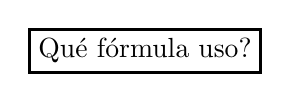
\begin{tikzpicture}
\node[draw, line width=0.04cm] at (8.5,2) {Qu\'e f\'ormula uso?};
\end{tikzpicture}
}

% ============================================================== 
%----------------------------------------------------------------
%----------------------------------------------------------------
\end{frame}

%________________________________________________________________(ult. col, 65)
% ========================== slide2 ============================= 
\begin{frame}
\frametitle{MRU}
% 
% -Paragraph1 
%----------------------------------------------------------------
%----------------------------------------------------------------
% -Idea1 
% ============================================================== 
 
{\huge                
\xmru
}

Desde 12:45 am hasta
19:55 pm han pasado:\\
{\tiny 
de 12:45 a 16:45 = 4 horas. \\
de 12:45 a 17:45 = 5 horas. \\
de 12:45 a 18:45 = 6 horas. \\
de 12:45 a 19:45 = 7 horas. \\
}

\begin{center}
{\huge + }
10 minutos
\end{center}

\fbox{7 y 1/6 horas!}.

% ============================================================== 
% -Idea2 
% ============================================================== 
 
% ============================================================== 
%----------------------------------------------------------------
%----------------------------------------------------------------
\end{frame}

%________________________________________________________________(ult. col, 65)
% ========================== slide3 ============================= 
\begin{frame}
\frametitle{MRU}
% 
% -Paragraph1 
%----------------------------------------------------------------
%----------------------------------------------------------------
% -Idea1 
% ==============================================================

%%%%%%%%%%%%%%%%%%%%%%%%%%%%%%%%%%%%%%%%%%%%%%%%%%%%%%%%%%%%%%%%
%%%%%%%%%%%%%%%%% Cajita de Texto sencilla %%%%%%%%%%%%%%%%%%%%%
\begin{center}
\fcolorbox{red}{white}{
\parbox[c]{5cm}{ % Reduced width to mitigate potential overfull hbox
1/6 
(en fracci\'on es m\'as f\'acil de manejar),
es porque 10 minutos es la 6 parte de 60 minutos.
}}
\end{center}
%%%%%%%%%%%%%%%%%%%%%%%%%%%%%%%%%%%%%%%%%%%%%%%%%%%%%%%%%%%%%%%%
%%%%%%%%%%%%%%%%%%%%%%%%%%%%%%%%%%%%%%%%%%%%%%%%%%%%%%%%%%%%%%%%

% ==============================================================
% -Idea3
% ==============================================================

Finalmente..

% ============================================================== 
% -Idea2 
% ============================================================== 
 
La distancia que separa a los dos destinos es:
{\large
\begin{equation}
x=
\left(1053\frac{\text{km}}{\cancel{\text{h}}}\right)
(7.16\cancel{\text{h}})=
7539.48~\text{km}
\end{equation}}

                                                             
% ============================================================== 
%----------------------------------------------------------------
%----------------------------------------------------------------
\end{frame}

%%%%%%%%%%%%%%%%%%%%%%%%%%%%%%%%%%%%%%%%%%%%%%%%%%%%%%
%%%%%%%%%%%%%%%  Tail  %%%%%%%%%%%%%%%%%%%%%%%%%%%%%%%
%%%%%%%%%%%%%%%%%%%%%%%%%%%%%%%%%%%%%%%%%%%%%%%%%%%%%%

\end{document}
%%
%% End of Beamer-ported file ==
%%
%% Modified 05-10-2008
